% !TEX root = NSF_SuperCDMS_SNOLAB_OPS.tex
%% people who build community and knowledge
%% around software?
%% The maintainers
%% Educopia
%% http://ivory.idyll.org/blog/2019-communities-of-effort.html#disqus_thread
%% https://blog.dnanexus.com/2018-01-29-analysis-commons-a-collaborative-approach-to-multi-omics-discovery/

%% describing data
%https://library.si.edu/research/describing-your-data-data-dictionaries
%https://figshare.com/articles/The_State_of_Open_Data_Report_2017/5481187/1
%https://www.usgs.gov/products/data-and-tools/data-management/data-standards
%https://www.fgdc.gov/standards/standards_publications/
%http://www.ddialliance.org/ metadata standards for social sciences
%https://www.rd-alliance.org/groups/data-type-registries-wg.html research data alliance, not focused on physics AFAIK but definitely useful
%https://access-data.trydiscourse.com/
% XDR, external data format!!
% https://tools.ietf.org/html/rfc1832.html#section-6
% and there is a python library for it, xdrlib

% Mom says all the cool kids are using smartsheets
% Liquid Planner has a free plan for teachers?  https://app.liquidplanner.com/space/202855/projects

% documentation is often overlooked but people need it the most
% https://opensourcesurvey.org/2017/

\section{Science-driven}
% How will the project outcomes fill well-recognized science and engineering needs of the research community, and advance research capability within a significant area or areas of science and engineering? What are the broader impacts of the project, such as benefits to science and engineering communities beyond initial targets, underrepresented communities, and education and workforce development? The project outcomes should address well-recognized science outcomes.

This project serves the immediate needs of researchers in the dark matter community and the experimental nuclear physics community by providing a common toolset for analyzing data in any format.

The PI expects that

\begin{itemize}
    \item Multiple research projects across the NSF directorate will be more productive because they can use existing, documented tools rather than building their own.  The PI intends to estimate this impact with citations from scientific papers.
    \item Increased involvement of undergraduate researchers in science analysis due to improved documentation and an extended support network.  The PI intends to measure this through undergraduate involvement in her own lab, community surveys, and tracking community forum data.
    \item Several example analyses will be publicly released, with accompanying documentation and support information for pre-requisite computing skills.  The intent is for these educational materials to be accessible to someone with no domain knowledge.  The PI believes these training materials will be an equitable training resource.
\end{itemize}


\subsection{Innovation}
% What innovative and transformational capabilities will the project bring to its target communities, and how will the project integrate innovation and discovery into the project activities, such as through empirical research embedded as an integral component of the project activities? Such research might encompass reproducibility, provenance, effectiveness, usability, and adoption of the components, adaptability to new technologies and to changing requirements, and the development of lifecycle processes used in the project.

A common limitation of data-analysis software that is entirely home-grown is that it does not scale as data grows and changes - a human has to update or rewrite the code if the requirements change substantially.

This library makes heavy use of existing libraries.  The benefit is that as those libraries improve and scale to larger data sets, this software inherits that improvement.  

In both cases, significant human effort is needed to adapt the software to changing data and needs.  But by leveraging well-supported, open-source libraries, the burden is shifted away from an individual scientist and towards an active community that is highly motivated to solve similar problems.  This library serves as sugar to allow scientists with many different data formats to take advantage of these popular libraries.

The danger to this approach is the same - if these libraries lose community support or focus on very different problems then this library will lose relevance over time.  To mitigate this risk, the PI is focusing on integrating with a library supported by the IRIS-HEP collaboration and with pandas, which enjoys extreme popularity in the data science community.

\subsection{Close collaboration among stakeholders}
% How will the project activities engage CI experts, specialists, and scientists and engineers working in concert with the relevant domain scientists and engineers who are users of CI?

The PI proposes to engage both cyberinfrastructure experts and the experimental nuclear physics community by (1) working closely with pilot experiments to build software that works effectively for scientists analyzing event-based data, (2) holding yearly workshops intended to foster interaction between the scientists using the software and cyberinfrastructure developers, and (3) attending conferences that will allow outreach to the scientific community (for example, the Low Energy Community Meeting) and the cyberinfrastructure community (for example, CHEP).

The PI has working relationships with scientists in the SuperCDMS collaboration and the XIA corporation, both of which are interested in exploring the proposed software as solutions to analysis needs.

In addition, the IRIS-HEP collaboration is interested in this work as it would extend their awkward-array library to a broader audience.  Awkward array was developed by Jim as part of DIANA/HEP (http://diana-hep.org,
OAC-1450377) and that effort will continue with IRIS-HEP
(http://iris-hep.org, OAC-1836650).  Collaborating with IRIS-HEP gives us access to experienced cyberinfrastructure developers who have focused on developing software suitable for terabyte-scale data.


\subsection{Building on existing, recognized capabilities}
% How will the project activities build on and leverage existing NSF and national cyberinfrastructure investments, as appropriate?

The proposed work builds on existing capabilities and communities in several ways:

\begin{itemize}
    \item \textbf{The PI proposes to use already-existing data description languages.}  The languages Katai Struct and the Data Format Description Langauage both have active communities and tools that work with data when provided a description.  Kaitai Struct is the target for the proposed work because (1) it is more human-readable than than the XML-based DFDL, and (2) Katai Struct generates code libraries that allow users to load their data into the programming environment of their choice; DFDL currently works by providing an XML or JSON equivalent of the binary data.  While this is a powerful approach because any language with an XML or JSON parser can now read the data, it also produces a secondary data file that is an order of magnitude larger than most binary files.  This makes DFDL, in its current state, unusable for scientists with gigabyte-scale data sets as it would make the required storage space for analysis prohibitively expensive.
    \item \textbf{The PI proposes to use already-existing infrastructure for the data-analysis library.}  Scientists who would like to avoid writing custom software to read their binary data can already use the Kaitai Struct compiler to generate libraries to read their data in python, C++, and a multitude of other languages.  The advantage is that there is substantial support documentation and an active community available for troubleshooting.  The disadvantage is that the current Kaitai Struct python compiler stores the data in a structure that does not provide adequate speed performance for gigabyte-scale data sets.  By improving the existing Katai Struct compiler software, we can build a science-ready analysis library and scientists can benefit from the existing community support and documentation.   
    \item \textbf{Use a supported and optimized data structure}  for the improvements to the Kaitai Struct compiler.  The ``awkward-array'' library was developed by DIANA/HEP and is now supported by IRIS-HEP and is part of a set of libraries designed to provide flexible data-analysis tools for the high-energy physics community.  The awkward-array data structure is optimized for fast queries on an event-based data set and as such is ideal for the majority of nuclear physics data.  By choosing this data structure as the target, we bring the optimized and convenient analysis environment of awkward-array to any scientist who describes their data with the Katai Struct language.
    \item \textbf{Provide analysis tools for the python environment and training materials that take advantage of the python ecosystem.}  Python is a popular analysis environment in the field of big-data and has enjoyed significant adoption in the scientific community; enough so that python support is compiled in the dominant high-energy physics software, ROOT, by default.  By providing a python library for data analysis, scientists can make use of a full ecosystem that supports data analysis: numpy for convenient array manipulation; scipy for fitting; matplotlib for producing publication-quality figures; and even numba for easy compilation of code that needs to run fast.  This entire environment is easily installed - even for users without administration privileges - through the Anaconda Python distribution.  There are many free and paid programming environments that are availble, notably the Jupyter environment.  Code written in this environment is particularly nice as a tutorial because it is rendered nicely on github, gitlab, and interactive notebooks can be opened in one click through binder.  By providing a small set of introductory documentation, scientists can benefit from the effort the python community has put in to lower the barrier for use.
    
\end{itemize}

\subsection{Project plans, and system and process architecture}
% For an "Elements" proposal, the Project Description should include a high-quality management plan. The proposal should include user interactions and a community-driven approach, and provide a timeline including a proof-of-concept demonstration of the key components. Software or data cyberinfrastructure services should be sufficiently described and follow industry best practices, including the architecture of the CI and the engineering process to be used for the design, development, documentation, testing, validation, and release of the software, its deployment and associated outreach to the end user community, and an acceptance and evaluation plan that involves end users. The description of the CI architecture and processes should explain how security, trustworthiness, provenance, reproducibility, and usability will be addressed by the project and integrated into the proposed system and the engineering process, and how adaptability to new technologies and changing requirements will be addressed by the project and built into the proposed system, as appropriate.

The timing of the proposed work is driven by the proposed, yearly workshops that focus on (1) teaching scientists how to use the tools to access their data, (2) working with scientists to perform their analyses in the python environment, (3) identifying improvements needed for the software to be easy to learn and useful in analysis, and (4) bringing developers into close contact with the science community using their tools.  Each workshop will result in an updated roadmap for the software.

Thus, the workshops - and software releases that include testing, documentation, and example analyses - are the primary milestones of the proposed work.

The work for each yearly cycle can be broken down into the following categories: development of basic computing skills learning material; development of the data-access library; planning and execution of the workshop; and a community-driven update of the roadmap.  See Table~\ref{tab:WBS} for details on who will perform this work.

The minimum requirements of the work determine the work plan and are the following:

\begin{enumerate}
    \item If students or staff move on to other positions, their replacements should be able to get up to speed in a month or less.
    \item Someone with no domain knowledge but reasonable persistence should be able to run the example analysis within a week.
    \item Someone with no domain knowledge but reasonable persistence should be able to analyze their own data within a month.
    \item A scientist who uses the access-data library to obtain a science result should know how to cite the software.
    \item A scientist experiencing trouble using the software should be able to determine how to get help quickly (within five minutes of searching).
    \item A scientist who wishes to improve the code should be able to quickly determine how to contact the developers and how to change, test, and push the code.
\end{enumerate}

The scope of the proposed software is relatively modest: copy an existing framework and adapt it so that it stores data in awkward-array structures rather than slower, dictionary structures.  The development and testing of this code will take time - but reference code for similar work exists, there is robust community support, and there is a developer guide that gives specific instructions for developers who wish to extend the existing Kaitai Struct code in this way.  The proposed work is feasible because it connects two libraries that are both designed for this purpose.

The majority of the proposed work is in making this software easy to use for scientists, and making it easy for the community to participate in the direction and development of the software.  This requires robust documentation for both users and developers.  Users will require installation instructions, instructions for using the library, and guidance on how to adapt the examples for their own analysis needs.  Developers will need additional documentation: instructions for changing the code and testing the code, and instructions and guidance on contributing their changes to the project.

To meet the minimum requirements, the workplan involves creating of initial documentation and an automated testing suite by the Professional Research Associate and example analysis created by the Master's student.

Undergraduates will begin either by working on new scientific computation skills or improving or adding to material of already-developed scientific computation skills.  Students who join the lab currently have two first projects to chose from: working through an introductory lab on water simulation, or working through an example analysis of gamma-spectroscopy data.  The students try to perform their work using existing documentation; the PI provides guidance when this is inadequate.  This provides an opportunity for students to design improvements and learn the basics of contributing to a code repository.  In addition to providing valuable training for the students, this process identifies gaps in the documentation that are often invisible to experts.

This initial work is expected to result in improvements and additions to web-accessible tutorial materials.  In addition, this training will provide a foundation that will allow the students to attempt the following actions:

\begin{itemize}
    \item Successfully follow a simple example analysis using the data-access library.
    \item Successfully follow a tutorial to make and share a change to the library documentation.
    \item Successfully follow a tutorial to make, test, and share a change to the library source code.
\end{itemize}

\begin{tabularx}{\textwidth}{XXX}
Work & Who & Notes \\
\toprule
Roadmap \& workplan development
& PI, PRA, Master's student
& \\

Basic skills materials 
& Undergrads
&  \\

Data-access library development
& 
& \\
code dev
& Professional Research Assistant
& this includes testing, user documentation, and dev documentation\\
contributing
& Professional Research Assistant
& this includes automated testing and contribution guidelines and instructions \\
example analyses
& Master's student
& \\
documentation testing
& Undergraduates, Master's student
& documentation testing may feed back into additional skill documetation \\

Workshop
& 
& \\
Recruiting
& PI
& \\
Organization
& Professional Research Assistant, Undergraduates
& \\
Pre-workshop analysis coordination
& PI, Master's student, PRA
& \\

Community-driven update of roadmap
& PI, PRA, Community
& \\
\label{tab:WBS}
\end{tabularx}

\begin{figure}[htb]
    \begin{center}
      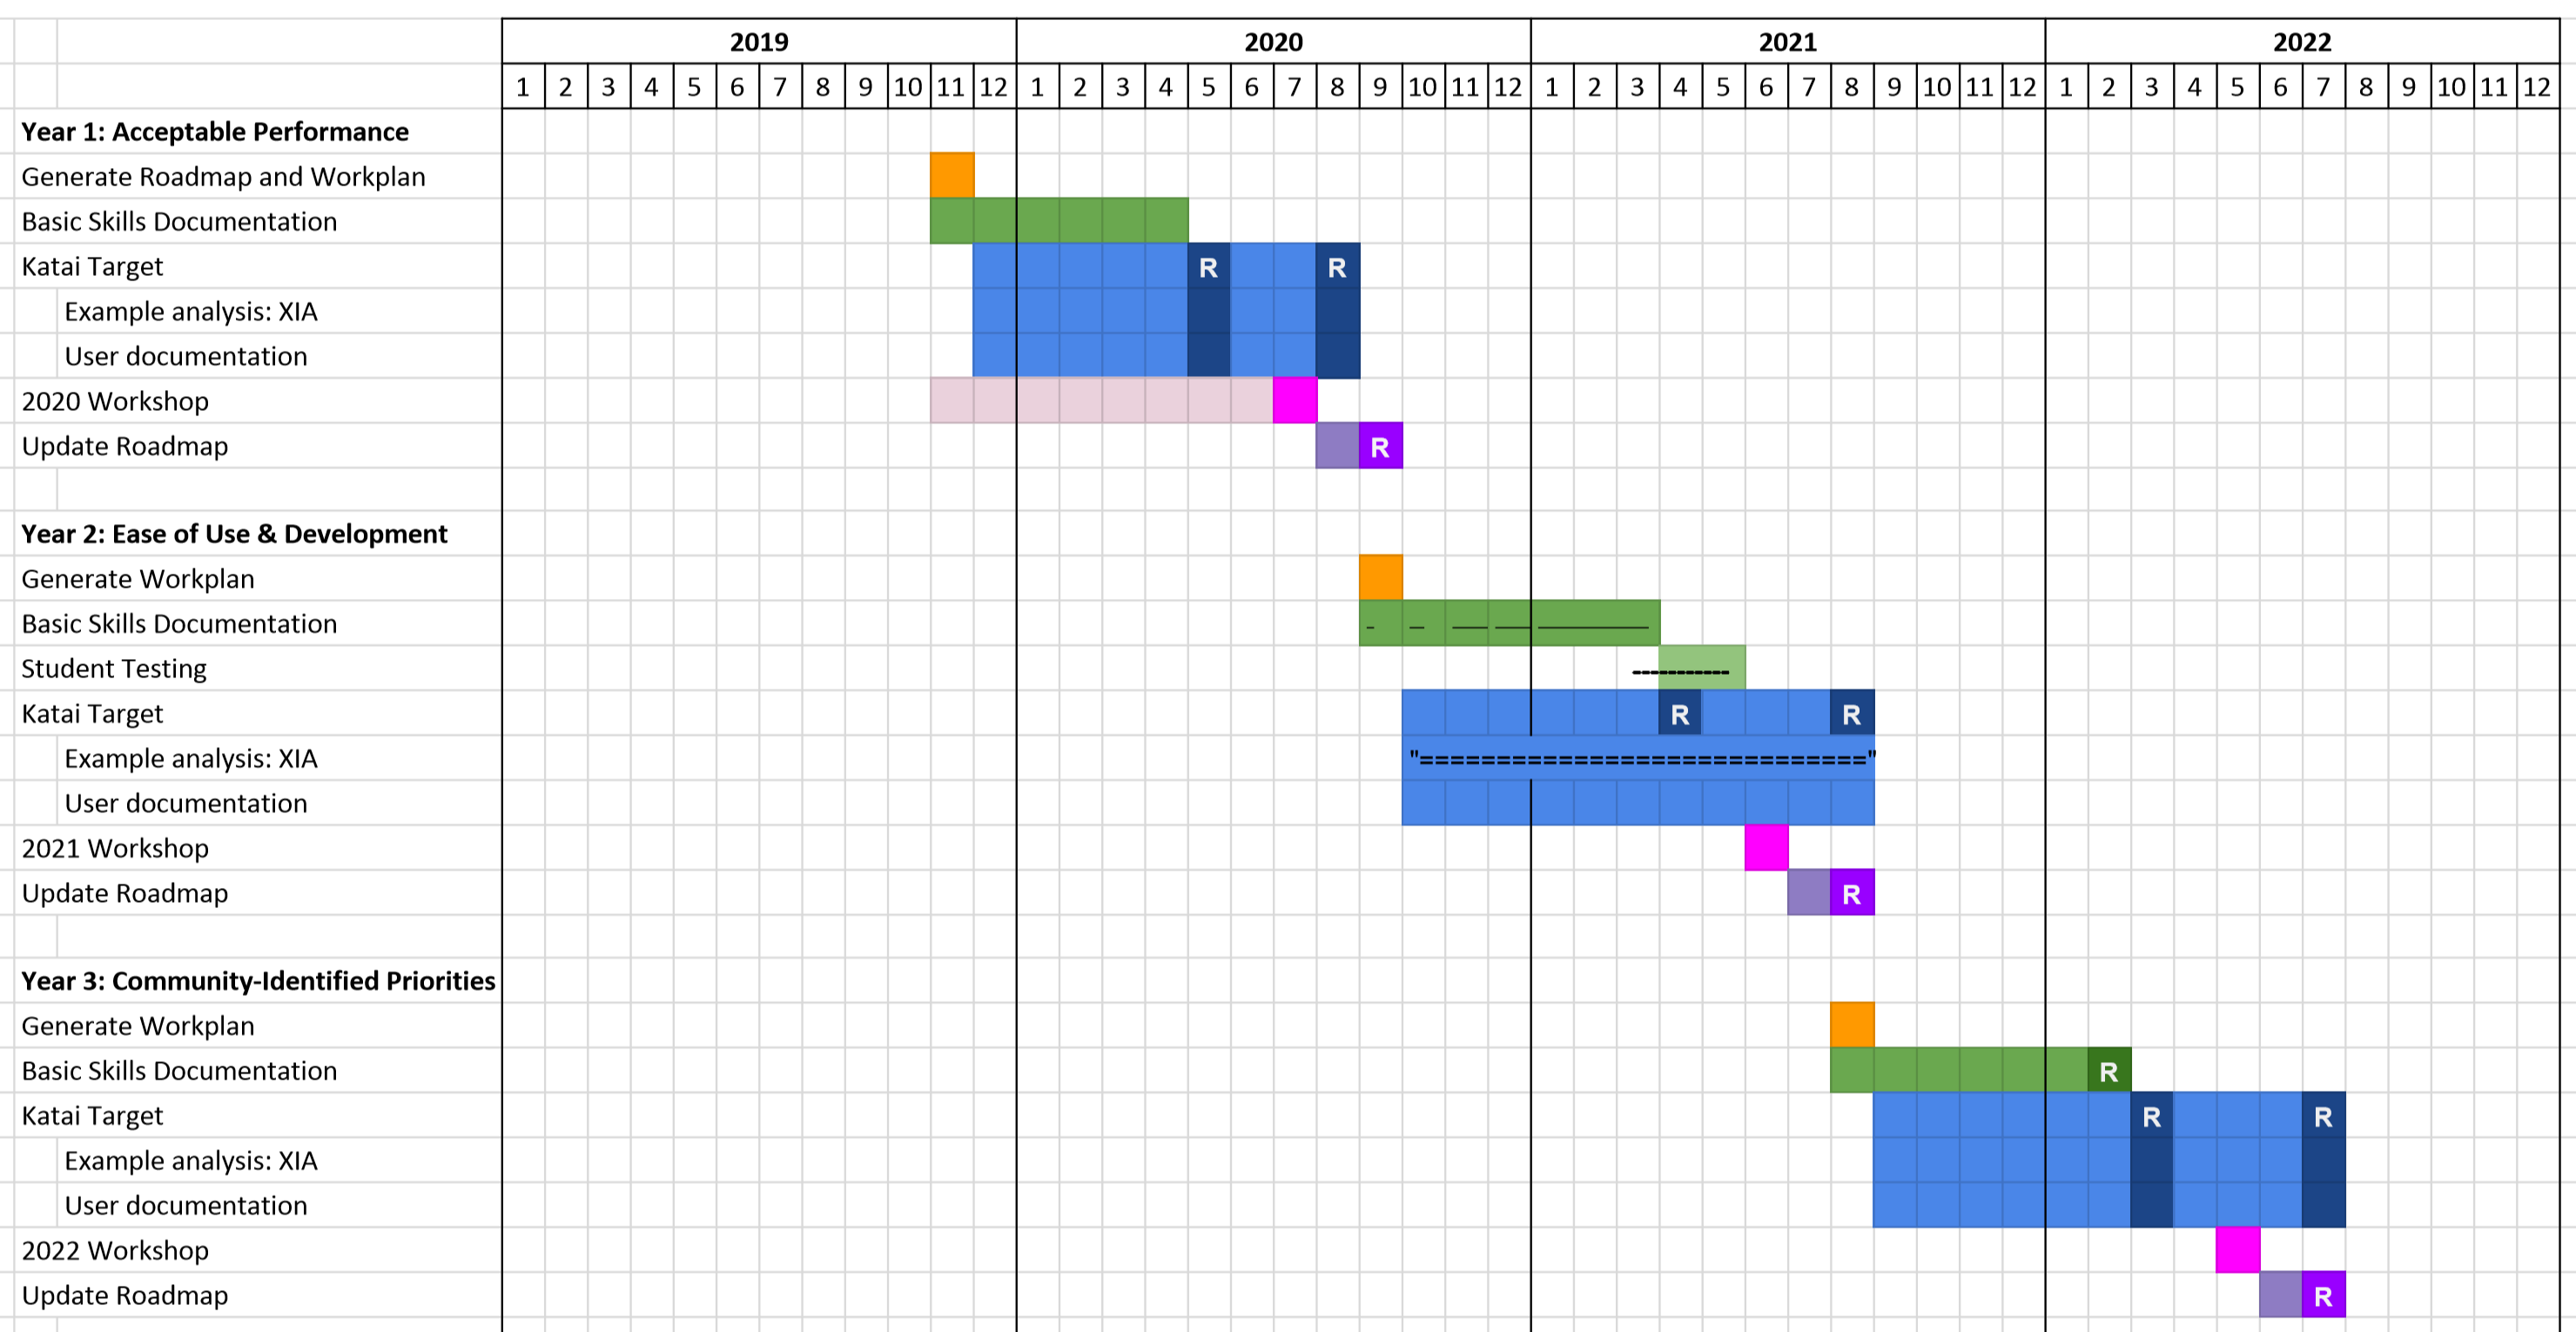
\includegraphics[width=\textwidth]{Figures/schedule1}
    \end{center}
    \caption{Schedule for the proposed work.}
    \label{fig:ops-schedule}
\end{figure}

\textbf{Architecture of the software:}
The architecture of the Kaitai Struct compiler that targets an awkward-array data structure will follow that of the existing Katai Struct software.  Implementing a Kaitai Struct compiler for a new language requires

\begin{enumerate}
    \item Writing a ``runtime library'' that provides a standard stream interface in the target language.  For example, one of the functions every language needs to have defined is a method that returns the size of the file or string stream.  By writing a ``size'' function for the language of interest that follows the Katai Struct API, the code generation becomes simpler.
    \item Writing a ``compiler'' that translates Kaitai Struct concepts, implemented in Scala, into the target language.
    \item Writing a test runner for the new language. 
\end{enumerate}

The proposed work targets the python environment, and there is already a Kaitai Struct python compiler.  The ``compiler'' for the python implementation, however, stores data in native-python data structures that provide inconveniently slow access to standard queries on large, gigabyte-scale data sets.  

However, the changes that need to be implemented to instead store the data in the faster awkward-array data structure are restricted to the compiler code.  The runtime library provides a convenient interface for reading data from a file or stream - this code only cares about the file system interface and does not need to change.  The python test interface will need to be updated as the access syntax for the data will change slightly.

Although there is opportunity for improving the speed of the data load, this development will instead focus on adhering to the existing format and style of Kaitai Struct.  The goal is to make the existing Kaitai Struct community useful to scientists who work with gigabyte-scale data sets; waiting for a few minutes for the data to load is not ideal but is typical of many locally-built solutions.  We can address the more-critical issue of rapid data queries while staying well within the existing framework of Kaitai Struct and intend to do so for the initial implementation of the software.

If we find that data-load times are a significant issue for the nuclear physics community then we will consider more substantial changes to the Kaitai Struct compiler and runtime libary.

\begin{lstlisting}
def [*size(self)*]:
    # Python has no internal File object API function to get
    # current file / StringIO size, thus we use the following
    # trick.
    io = self._io
    # Remember our current position
    [*cur_pos = *]io.tell()
    # Seek to the end of the File object
    io.seek(0, SEEK_END)
    # Remember position, which is equal to the full length
    [*full_size = *]io.tell()
    # Seek back to the current position
    [*io.seek(cur_pos)*]
[*return full_size*]
\end{lstlisting}

\begin{lstlisting}
uint64_t kaitai::kstream::[*size()*] {
    std::iostream::pos_type [*cur_pos = *]m_io->tellg();
    m_io->seekg(0, std::ios::end);
    std::iostream::pos_type [*len = *]m_io->tellg();
    [*m_io->seekg(cur_pos)*];
    [*return len*];
}
\caption{The details of this code are not important.  What is significant is the name of this function, size(), and its behavior: find and report the size of the file, without changing where we are in the file.  The Katai Struct compiler for both C++ and python can use the ``size()'' function rather than including these language-specific stream commands, making the compiler code more readable.}
\end{lstlisting}

\textbf{Architecture of the user documentation:} User documentation should make it possible for users with little to no domain knowledge to use the data-access library for science.  Documentation for the use of the library will be stored as text files in the repository with the code.  The files will be written in markdown syntax to improve their readability; this will also render them nicely on cloud-based repository hosts such as github and gitlab.  The following documentation will be provided:

\begin{enumerate}
    \item How to get help with questions or issues about the library.
    \item How to install the library and its dependencies.
    \item An overview explaining what the user will need to provide (data and a description of the data) and what the library will provide (software to read that data).
    \item A tutorial walking through the use-case of a scientist looking at simple data with a custom format.
    \item Links to additional resources detailing more complex data formats and more complex analyses.
    \item Citation guidelines.  
\end{enumerate}


\textbf{Architecture of the developer documentation.}  Documentation intended to facilitate development of the code will be stored in the repository alongside the code.  Text files referenced in the top-level README file will detail, for every repository,

\begin{enumerate}
    \item How to install, develop, and test the code for individuals who wish to make changes.  
    \item How to contribute changes back to the project.  This will provide instructions on the version control practices used by the repository maintainers and instructions for implementing the tests required for changes to be considered for merging with the main code base.
\end{enumerate}

\textbf{Architecture of the basic scientific computing skills documentation:}  Documentation of basic computational skills and concepts will have several possible forms: (1) Text and images, (2) tutorial videos, (3) jupyter notebooks, (4) printable images that illustrate a focused concept, and (5) links to recommended resources such as Software Carpentry tutorials.

All materials will be licensed with  a permissive, open-source license such as CC-BY or MIT.  The source for all the materials will be publicly available through a public host such as github or gitlab and will be archived on a content-tracker such as the Open Science Framework or Figshare.  Videos will be released on YouTube and licensed CC-BY.

All materials will be disseminated using a static site generated by Antora.  Antora is specifically designed for documentation and allows a user to specify a set of repositories containing text files formatted in the Asciidoc markdown language to build a single, searchable documentation site.  Because Antora generates a static site, free hosting services are readily available.  This solution allows my students to focus on creating material to explain core concepts and practice interacting with version control rather than spending time wrestling with web development.

The topics students choose to document are largely student-led, with some guidance from the PI.  Spring 2019 marks the inception of this project, and the concepts chosen by students for illustration have focused on (1) tutorial-format guide for installing python and running a basic python-based analysis of gamma spectroscopy data, (2) instructions for using a docker container to simplify installation of a complex software environment, and (3) a poster explaining what an executable file is.

Documentation that will be provided in this format alongside the scientific computing resources will include

\begin{enumerate}
    \item instructions on where to get help with the material and how to provide feedback and and file bug reports
    \item instructions for those who wish to contribute to the documentation
    \item instructions for the deployment of the documentation
\end{enumerate}


\textbf{Engineering processes:}
% design, development, documentation, testing, validation, and release of the software
% and
% description of the CI architecture and processes should explain how security, trustworthiness, provenance, reproducibility, and usability will be addressed by the project and integrated into the proposed system and the engineering process
A primary goal of the proposed work is to build software that can be supported and maintained by the community.  A primary risk of the proposed work is staff turnover and associated loss of knowledge and onboarding time.

The software design, development, documentation, and testing work together to make it easy for the community to contribute to the software development - a goal that mitigates turnover risk as well.

The design process of the software will start with project documentation that describes (1) use cases, (2) requirements, (3) assumptions, (4) key decisions, and (5) definitions.  Such documentation is particularly useful for programmers who lack experience in experimental nuclear physics data analysis and makes it easier for skilled experts to contribute to the project.  This documentation also serves as a way to focus community discussions into defining a minimum useful scope for the software.

The development of all software in the PI's lab is done using version control software (git) and a central ``repository server'' that everyone interacts with.  Cloud-based servers such as github and gitlab are used because they are easy to use, provide robust backups, and also serve as a platform for dissemination and collaboration.

The PI's approach to version control and software releases prioritizes (1) easy-to-get, working code and (2) rapid updates.  This is implemented by building end-to-end tests and configuring automatic test running triggered by any changes to the repository.  Rather than insisting on a specific release cycle, developers are encouraged to put their changes on the public, master branch if their code is non-breaking.  Code on the public, master branch MUST pass all tests.  Semantic versioning will be used to alert users to breaking changes.

Work that breaks tests MUST be maintained on a separate ``branch'' that is publicly available but that will only be available to users by explicit action.  Instructions for developing code on such a branch will be included in the contributions documentation.

The key to this type of development is building simple end-to-end tests, implementing an automated testing framework, and investing heavily in documentation and testing of that documentation up front.  This development strategy works well for the proposed project because the software goal is already well-defined and the initial plan for implementation - leverage the existing Kaitai Struct framework as much as possible - is clear.  In addition, this development strategy is well-supported by community solutions and the organization of the PI's lab:

\begin{itemize}
    \item end-to-end testing of python code - and even tutorial notebooks in jupyterlab format - enjoy a thriving ecosystem in Python.
    \item many automated testing frameworks are designed specifically to support developers using cloud-based repository hosts such as github and gitlab; many are freely available to open-source projects.
    \item novices are always on hand to test documentation.  The PI maintains a group of approximately six students, many of whom have minimal experience with scientific computing.  Giving them goals such as: work through this example analysis and obtain a similar plot exposes conceptual gaps and problems with the documentation while providing excellent training for the student.  In addition, students have responded well to the opportunity to make a substantive contribution to the lab.
\end{itemize}

In summary, the proposed code development will be strongly tied to documentation, automated testing, and documentation testing.

%\subsubsection{Security}

\subsubsection{Trustworthiness}
End-to-end tests of the software will include tests where the outcome is known.

\subsubsection{Provenance}
All releases will be archived with their own DOIs on Zenodo.  Guidance to cite the version of the software used will be included in the top-level README of all releases and posted on all related websites.

\subsubsection{Reproducibility}
End-to-end tests of the software will completely define all inputs, including a reference data set, and compare the output to reference products such as histograms.  The PI acknowledges that this is in no way a complete test of reproducibility but feels that it will be a useful starting point.  

Instructions for system setup will be included in the documentation.  Full or partial system specifications are required for automatic test running and will be versioned together with the rest of the code.  The most popular of these, Docker, will be used.  More complete system specifications as provided by Nix and Guix will be considered if need arises for more complete reproducibility.

\subsubsection{Usability}
For the proposed software, usability consists of several scenarios:

\begin{tabularx}{\textwidth}{XX}
    Can a scientist easily use this code to do data analysis on a custom-format data set? & \\
    \toprule

    Is the scientist aware that this software exists?  Can the scientist find the software easily even if all they recall is a vague description?
    & Publications citing DOIs hosted on Zenodo with published preprints; well-indexed project website; open development on github, gitlab; indexed on python library repositories where appropriate \\
    Can the scientist install the software on their analysis computer easily, with or without root access?
    & Installation documentation; testing of installation documentation by novices; review of systems that need installation support at workshops \\
    Does the software apply itself well to this particular analysis need?  Can the scientist see how to use the software in their analysis?
    & Example analyses; testing of example analyses by novices; creation of a ``now you try'' document to test effectiveness. \\
    Does the scientist know where to get help or discuss issues with the software?
    & All documentation and code will contain a header directing users to the project forum and repository issue tracking. \\


Can an interested individual contribute to the development of the software easily? & \\
\toprule

    Is there a clear description of the requirements and purpose of the software so that developers can decide if they'd like to participate?
    & Requirements documentation and a description of use cases will precede all programming work and will be versioned with the rest of the code.\\
    Is it clear where to get help or discuss the code?
    & All documentation will link to the forum and the repository issue tracker.  The forum will be configured for web crawlers to maximize its discoverability.\\
    Are there clear and complete instructions on testing the software locally?
    & Local and remote testing infrastructure is as high in priority as the initial development of the code; documentation will be written as part of the first efforts.  Students will test these local development instructions.  Instructions may reference the scientific computing documentation.\\
    Are there clear and complete contribution instructions?
    & Contribution instructions will be developed with high priority once there is an initial passing test, even before there is functioning code.  Students will test these contribution instructions.  Instructions may reference the scientific computing documentation.\\
\end{tabularx}


\subsubsection{Adaptability}
The proposed software intends to support scientific analysis of gigabyte-scale data for the coming decade.

The benefits of the proposed software, compared to the current, group-driven methods, are increased access to scientific analysis through ease of use, quality documentation, and community support.  And improved return on invested maintenance time, since effort on a common set of tools can benefit many scientists.

Another advantage of the proposed software is that it leverages existing, well-supported projects to deliver science-ready software.  Adaptations to changing data needs and opportunities can potentially come from efforts outside nuclear physics.

There is always the possibility that these dependencies could be abandoned.  Archives of all dependent software will be made as a safeguard against this.  Other risk mitigation the PI will pursue is significant investment in automated testing and documentation, particularly interface documentation.

\subsection{Deployment and user outreach:}
A key component of the user outreach will consist of annual workshops designed to promote hands-on use of the software and close collaboration with the software developers.  To maximize the effectiveness of these workshops,

\begin{itemize}
    \item Participants will be contacted in advance to begin early coordination of the analysis they're interested in doing with the data-access library
    \item Communication before and after the workshop will be encouraged through the maintenance of an open forum
    \item Prototype software will be released along with installation documentation, an example analysis, and contribution documentation prior to the workshop and tested by novices
    \item Discussion of the community roadmap will be integrated into the workshop and a new release of the roadmap will follow each workshop
    \item The conference will be registered on the Open Science Framework, providing an archived record of material prepared by participants.
\end{itemize}

Deployment of this software will use common open-source channels such as github, gitlab, and python package indexes such as PyPI and Conda.  Github and Gitlab both provide static page serving for projects.

Project communication will use the built-in issue tracking provided by repository hosts and open forum software such as Discourse.  Live-chat is not an anticipated need, but if it becomes clear this would be useful then the PI will consider using freely-available chat services such as Slack, Zulip, or Gitter.

Deployment of the software will also happen through academic channels such as preprint servers, project releases on the Open Science Framework, and/or Figshare.



\subsection{Acceptance and evaluation:}

Community adoption of this software is central to the success and broader impact of this project.

The simplest evaluation metrics of community adoption and use will be (1) citations of software in peer-reviewed scientific papers and (2) the number of contributions to the code from developers outside the PI's group.

Additional metrics that may provide useful information could include: (a) number of downloads from the Zenodo or gitlab site and (b) quantity of interactions on the issue tracker and forum.

The PI intends to use interviews to understand how the software meets (or not) the needs of the community.  The yearly workshops will provide an ideal setting for such discussions.  In addition, a standing feedback survey will be linked from the project page to capture responses from the people who have the time and willingness to share.

This feedback will directly inform decisions about priorities and have an official outlet in the release of an annual roadmap.  Discussion and contribution to the roadmap will be open to the community and will begin at the yearly workshop.


\section{Deliverables}
% Does the proposed project clearly articulate the services and capabilities to be delivered, and how they are to be delivered? NSF encourages exploration of various delivery mechanisms, including but not limited to, those leveraging eXtreme Science and Engineering Discovery Environment (XSEDE), leadership-class computing resources, OAC Software Institutes, Big Data Regional Innovation Hubs, individual organizational resources, and well-known public and private cloud services.

\section{Metrics}
% Does the proposed project clearly articulate quantifiable metrics for development and delivery of the services and capabilities to be delivered by the project, and for the anticipated community adoption and usage? Are quantitative metrics with targets identified for each year of the award? These should be simple but should also clearly show what the project will accomplish each year, the impact on science, and the breadth of the user community.
The simplest evaluation metrics of community adoption and use will be (1) citations of software in peer-reviewed scientific papers and (2) the number of contributions to the code from developers outside the PI's group.

Additional metrics that may provide useful information could include: (a) number of downloads from the Zenodo or gitlab site, (b) quantity of interactions on the issue tracker and forum, and (c) materials provided by data-sharing platforms that educate scientists on data-description languages.

Another informal metric of community support is how many scientists apply to the yearly workshop who are not actively solicited by the group and individual interviews with scientists using the software.

\subsubsection*{Year 1}
An initial release of the improved software and the XIA library is made.  Both have basic testing coverage, are tested automatically upon commit, and have initial guidelines for contribution.  An initial release of the skills documentation has been made.
\begin{itemize}
  \item A whitepaper is published describing data description languages and giving use-cases
  \item No citations of the software library are expected from peer-reviewed science results in year 1.
  %\item The Open Science Framework and Figshare are contacted.  We find out if they're interested and if so, get a contact person.
  \item Between 15 and 20 scientists register for the Data Access workshop.  These scientists are expected to predominantly come from the nuclear physics community.  The PI expects all attendees to register after specific invitation.
  \item Between 2 and 5 scientists register projects with the Open Science Framework or similar platform to work on analysis of their data collaboratively
  \item An initial release of the improved software and the XIA library is made.  Both have basic testing coverage, are tested automatically upon commit, and have initial guidelines for contribution.
  \item Inexperienced students who try to follow the analysis tutorial are able to find answers to some of their questions but most are expected to be unable to complete the tutorial without expert assistance
  \item Interviews with scientists attending the workshop show that out of ten scientists: approximately two find the software useful as-is for their analysis work; approximately five would find the software useful but do not plan to use it because of solvable issues; and approximately three do not plan to use the software either because it is not useful to them or because their issues with the software cannot be easily addressed.
\end{itemize}

\subsubsection*{Year 2}
The highest-priority improvements as identified by the community roadmap are released.  The contribution guidelines and instructions are well-tested.   The most common failings of the skills documentation have been addressed. 

\begin{itemize}
  \item At least one peer-reviewed science result cites the data-access library.
  \item Between 15 and 20 scientists register for the Data Access workshop.  Some diversity of discipline is expected, although most are expected to predominantly come from the nuclear physics community.  The PI expects one or two attendees to find out and register for the conference from someone outside the group and for most to register after specific invitation.
  \item Between 3 and 7 scientists register projects with the Open Science Framework or similar platform to work on analysis of their data collaboratively
  \item  There has been at least one request for an improvement or feature from the community that has been either fixed by my team or another contributor.
  \item  Inexperienced students who try to follow the analysis tutorial get stuck on these issues less frequently.  Most are able to complete the tutorial without expert assistance but are unable to make significant progress on the ``now you try'' analysis tutorial without expert assistance.
  \item Interviews with scientists attending the workshop show that out of ten scientists: approximately four find the software useful as-is for their analysis work; approximately four would find the software useful but do not plan to use it because of solvable issues; and approximately two do not plan to use the software either because it is not useful to them or because their issues with the software cannot be easily addressed.
\end{itemize}

\subsubsection*{Year 3}
The highest-priority improvements identified on the road map for the core library are released.  The contribution guidelines and instructions are well-tested.  The basic-skills documentation has resources or recommends resources that address most of the questions that arise when inexperienced students try to follow the analysis tutorial.  

\begin{itemize}
  \item At least five peer-reviewed science results cite the data-access library.
  \item Between 15 and 25 scientists register for the Data Access workshop.  Some diversity of discipline is expected, although most are expected to predominantly come from the nuclear physics community.  The PI expects at least three attendees to find out and register for the conference from someone outside the group and for most to register after specific invitation.
  \item Between 5 and 10 scientists register projects with the Open Science Framework or similar platform to work on analysis of their data collaboratively
  %\item The highest-priority helper code is close to stable.  The contribution guidelines and instructions are well-tested.  There has been at least one request for an improvement or feature from the community that has been either fixed by my team or another contributor.
  \item There has been at least five requests for an improvement or feature from the community that has been either fixed by my team or another contributor.
  \item Inexperienced students can independently find answers to most of their questions when following the analysis tutorial.  Most students still need expert help on the ``try your own'' analysis tutorial but find it easier to formulate their questions
  \item Interviews with scientists attending the workshop show that out of ten scientists: approximately six find the software useful as-is for their analysis work; approximately two find the software useful as-is but would very much like to see one or several non-trivial issues addressed; and approximately two do not plan to use the software either because it is not useful to them or because their issues with the software cannot be easily addressed.
\end{itemize}


\section{Sustained and sustainable impacts}
%The Project Description should address how the project outcomes and its activities will have long-term impacts, and how these will be sustained beyond the lifetime of the award, as appropriate. Manuals and tutorials for using the developed CI should be delivered to the community. Software or data cyberinfrastructure services must identify the intended license to be used for the released CI, and the justification for the choice of this license. PIs who have been previously funded under previous CI awards should show quantifiable evidence of the use, impact and sustainability of the previously funded work (and include a citation to the published CI in their biographical sketches as one of their relevant products, if appropriate).

The goal of the proposed work is to significantly increase the accessibility of scientific data analysis on custom-format binary data.

The proposed work will not eliminate the need for developing custom software within institutions and groups - but the project will provide a common toolset that will work for the majority of gigabyte-scale, event-based analysis despite the lack of a uniform data format.  The success of this project is expected to

\begin{itemize}
    \item Reduce redundant time spent on writing custom data-access software
    \item Reduce experts' time spent fighting with existing software during analysis
    \item Significantly increase the involvement of students in the science-analysis phase of research
    \item Improve the reproducibility of science results 
    \item Allow software development to occur in an environment where credit for this often-invisible work is possible
\end{itemize}

The success of this project depends on significant community involvement; the PI believes that the flexible nature of the proposed software, its immediate need for many in the community, and the community-building work of the grant can achieve this goal.

The plan for long-term sustainability of this project is twofold.  (1) The scope of the proposed software is small and the PI expects this software to be in a mature state by the end of these funds.  Therefore the project is expected to require less effort from the core development team.  (2) It is expected that the work proposed will build a broad community of users and developers who will continue to support the software because it is directly useful to their science goals.

In addition to hoping that the community developed during the course of this funding will be able to maintain the software at a usable level, the PI will investigate possible support from organizations like NumFOCUS as well as the Open Science Framework and Figshare. 